%!TEX program = xelatex

\documentclass[UTF8]{ctexbeamer}

\usepackage{bookmark}
\usepackage{minted}
\usepackage{fontspec}
%--------------------------%

\setmonofont{Consolas}

%--------------------------%

\title{Aminer调研报告}
% \subtitle{测试——Testing}
\author{王清雨}
% \institute{
%     \inst{1}
%     \zihao{6}{联创团队 Web组}
% }

\subject{Computer Science}
\bibliographystyle{apalike}

%--------------------------%
\usetheme{Darmstadt}
\usecolortheme{wolverine}
\begin{document}

\maketitle
\frame{
    \tableofcontents
}

%--------------------------%

\AtBeginSubsection[]
{
    \begin{frame}
        \frametitle{目录}
        \tableofcontents[currentsection,currentsubsection]
    \end{frame}
}

%--------------------------%

\section{组织架构}
\frame{\sectionpage}

\subsection{概述}
\begin{frame}
    \frametitle{概述}


    从\cite{tang2008arnetminer}中可以看到如下图所示的架构,主要有以下几部分组成:
    \begin{itemize}
        \item {\heiti 获取信息}\textit{Extraction}
        \item {\heiti 整合}\textit{Integration}
        \item {\heiti 存储与访问}\textit{Storage and Access}
        \item {\heiti 建模}\textit{Modeling}
        \item {\heiti 搜索}\textit{Search Services}
    \end{itemize}
\end{frame}

\begin{frame}
    \frametitle{架构图}

    \begin{figure}[h]
        \caption{Architecture}
        \centering
        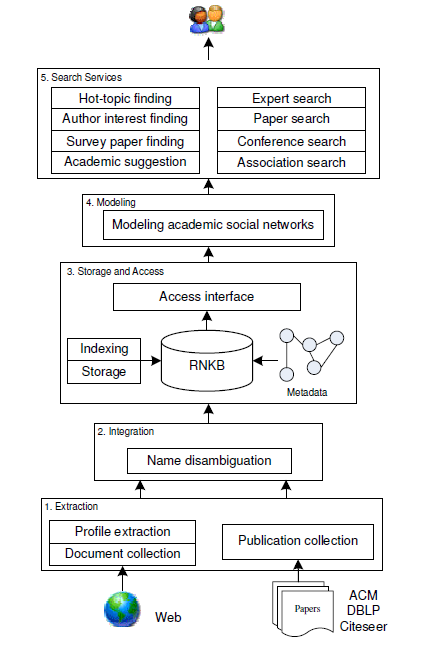
\includegraphics[width=0.4\textwidth]{assets/figures/arch.PNG}
        \label{fig:arch}
    \end{figure}

\end{frame}

\subsection{架构发展历史}
\begin{frame}
    \frametitle{Aminer是如何一步步成为今天的样子的}
    \begin{itemize}
        \item{2006年6月}
              信息提取,学者、论文、会议搜索
        \item{2006年8月}
              重写上述功能
        \item{2007年7月}
              添加学者研究兴趣、关联搜索(\textbf{\textit{Association search}})、\textbf{\textit{survey search}}?
        \item{2008年4月}
              查询理解(\textbf{\textit{Query understanding}})、新的搜索界面、日志分析
        \item{2008年11月}
              图搜索、主题挖掘(\textbf{\textit{Topic mining}})
        \item{2009年4月}
              信息编辑、开放资源
        \item{2009年12月}
              学术统计数据(\textbf{\textit{Academic statistics}})、用户反馈、精细化排名
    \end{itemize}

\end{frame}
%--------------------------%

\section{特点}
\frame{\sectionpage}

\subsection{功能}
\begin{frame}
    \frametitle{概述}

    \begin{itemize}
        \item 自动从互联网获取学者信息
        \item 将获取到的信息整合入现有数据库的网络中(不同来源的信息如何统一)
        \item 对整个学术网络进行建模
        \item 为学术网络提供搜索服务
    \end{itemize}

\end{frame}
\begin{frame}
    \frametitle{学者、文献搜索}

    Aminer 提供快速,精确的搜索服务。以学者搜索为例,系统会按照学者的论文数、被引用数、h-index等指标排序
    并且能准确地区分\textbf{同名}的不同学者。

    而在论文搜索中,Aminer 不仅仅能根据文章名进行搜索,还可以搜索与某一特定主题对应的论文。例如:直接搜索\textit{Data
        Mining}就会出现数据挖掘领域的杰出论文。
    %TODO: figure

\end{frame}

\begin{frame}
    \frametitle{学者关系}

    Aminer 能够从学者间的合作关系及其他一些数据来推断学者间的关系,例如:两位学者是否有师生关系。
    \cite{wang2010mining}
    %TODO: figure


\end{frame}

\begin{frame}
    \frametitle{学术趋势}

    Aminer 根据所拥有的数据,向用户展示了各领域的随时间的发展趋势,并根据引用数等指标给出了各个时间段各领域的代表性论文。

    %TODO: figure

\end{frame}



%--------------------------%

\section{后台技术}
\frame{\sectionpage}

\subsection{数据获取}
\begin{frame}
    \frametitle{概述}

    Aminer 采用一种类似\textbf{通用爬虫}的方法来获取学者的相关数据。\cite{tang2008arnetminer}

    {\songti 数据获取分为两个部分,\textbf{处理}和\textbf{CRF model}}

    {\zihao{5} 还有一些论文还没有读完}


\end{frame}
\begin{frame}
    \frametitle{处理\textit{Process}}

    处理分为三步:
    \begin{itemize}
        \item 有关页面识别
        \item 处理
        \item 提取
    \end{itemize}

    \textbf{有关页面识别:}先通过搜索引擎获取到一系列网页,然后通过二分类分类器\textit{(Binary classifier)}识别其中的学者主页。分类器采用支持向量机\textit{(Support Vector Machines)}作为分类模型。


    \textbf{处理:}先将文字划分为\textit{(token)},再给它们打上标签,每个标签对应一种学者的一个\textit{property}


    \textbf{提取:}从打好标签的数据中提取出需要的信息


\end{frame}
\begin{frame}
    \frametitle{CRF-Model}

    Aminer 使用 Conditional  Random  Fields\textit{(CRF)}来作为标记\textit{(tagging)}模型,模型会匹配所获取到的数据中学者的信息,如下图:

    \begin{figure}[h]
        \caption{features}
        \centering
        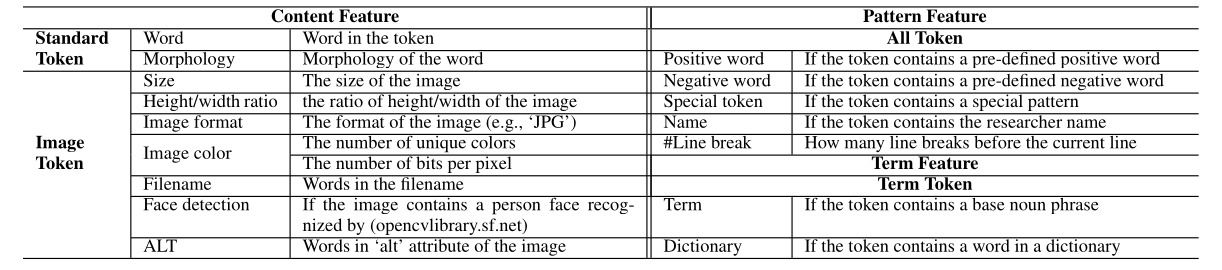
\includegraphics[width=\textwidth]{assets/figures/crfmodel.PNG}
        \label{fig:crfmodel}
    \end{figure}

\end{frame}
\begin{frame}
    \frametitle{遇到的挑战}

    鉴于原来对数据的爬取都是基于特定的数据集(如同一个网站),是否存在一种通用的爬虫,能够适用于所有的网页 \cite{tang2008arnetminer}

\end{frame}


\subsection{重名问题}
\begin{frame}
    \frametitle{Name Disambiguation}

    重名问题\textit{(Name Disambiguation)}指如何区分两个具有相同姓名的学者是否是一个人的问题(当然不局限于姓名)。

    这个问题是一个困难的、很久没有良好的解决方案的问题,在学术上也有诸多讨论,有多种不同的解决方案,但都不是很完美。

\end{frame}

\begin{frame}[allowframebreaks]
    \frametitle{解决方案}

    如何判断两篇具有姓名相同的作者的论文是否为同一作者所著?

    根据两篇文章是否有相同的引用、是否有相同的合作者、是否有相同的出版处、是否有相似的标题、是否出现在同一主页上等等关系建立一个概率模型,从而通过机器学习算法来判断是否是同一学者所著。\cite{wang2011adana}

    具体内部的模型及原理还需要更深入的研究。

    \begin{figure}[h]
        \caption{model}
        \centering
        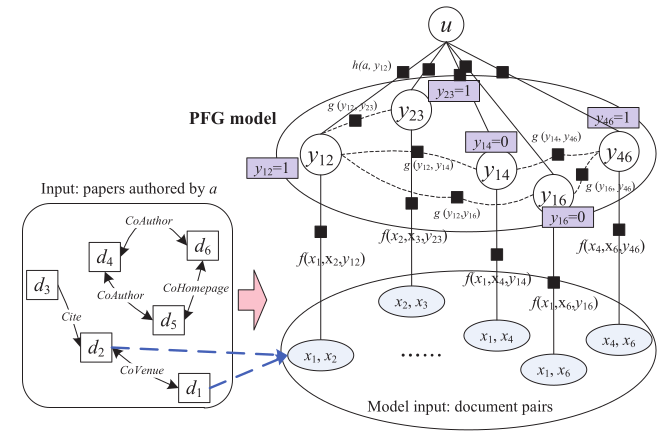
\includegraphics[width=0.8\textwidth]{assets/figures/pfgmodel.PNG}
        \label{fig:pfgmodel}
    \end{figure}

\end{frame}


\subsection{建模}
\begin{frame}[allowframebreaks]
    \frametitle{社交网络分析\textit{Topic-based} social influence analysis}
    社交网络\textbf{\textit{(Social network)}}的建模、分类及其内部关系,提出了\textbf{Topical Affinity Propagation}用来对社交网络进行建模。最终能够找到一个topic下最具代表性的节点,同时发现节点对周围节点的影响。
    \cite{tang2009social}

    如何对网页上的链接进行分类和如何量化链接的影响力
    \cite{tang2009topic}
    \begin{figure}[h]
        \caption{topical factor graph model}
        \centering
        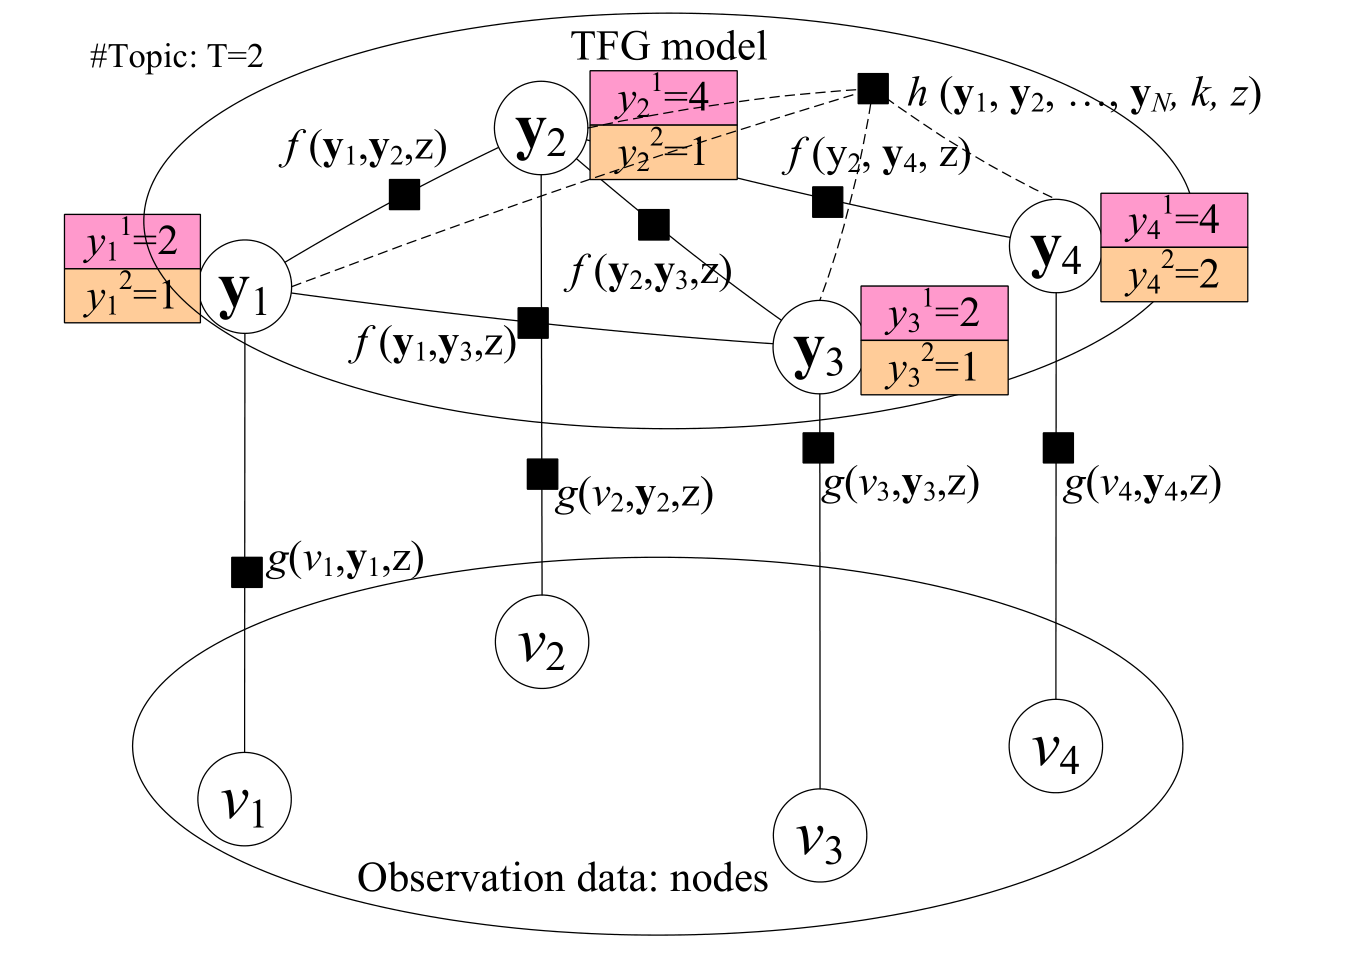
\includegraphics[width=0.8\textwidth]{assets/figures/model1.png}
        \label{fig:model1}
    \end{figure}


    如何将导师、学生关系从合作关系中提取、挖掘出来,并给出一种学习方法,用来提升提取的效果。

    论文\cite{tang2009topic,yang2010social,wang2010mining}中给出的是如今 Aminer 所做的事情的简化版。

\end{frame}

\begin{frame}[allowframebreaks]
    \frametitle{社交网络排名\textit{Topic-based heterogeneous ranking}}
    建立了一种新的建模方式\textit{Author-Conference-Topic(ACT) model},能够同时对论文、作者、出版物进行建模,还采用\textit{Random walk framework}来加强排名\textit{ranking}\cite{tang2008topic} 
    

\end{frame}


\subsection{搜索}
\begin{frame}
    \frametitle{搜索}

    在搜索方面,Aminer 采用了classical的方式\cite{tang2008arnetminer},因为已经足够成熟并且表现良好。

\end{frame}

%--------------------------%

\begin{frame}[allowframebreaks]
    \frametitle{参考文献}

    \bibliography{papers}

\end{frame}
\end{document}